\chapter{The Software Heritage Graph}%
\label{chp:swh-model}

% This chapter describes the abstract data model of the Software Heritage
% archive.

\section{Canonical Software Artifacts}%
\label{sec:swh-artifacts}

The Software Heritage archive is continuously ingesting software artifacts from
a wide array of sources, including different VCS and package managers that
each have their own internal data model. The main purpose of the Software
Heritage data model is to provide a generic structure in which the individual
object types specific to each system can be mapped to abstract concepts. For
example, Git ``commits'', SVN ``revisions'' and Mercurial ``changesets'' all
correspond to the same idea of a frozen state of the source tree, and thus they
are all \emph{canonicalized} as a single type of artifact that we call
``revisions''.

By stripping the implementation peculiarities of the individual data sources,
the artifacts are boiled down to a purely abstract form. This unifies the
representation of all the artifacts stored in the archive, which is
particularly interesting for research: since all the artifacts are already
stored in canonical form, we can provide a uniform interface for researchers
to study artifacts coming from a variety of different sources. This isolates
the complexity of handling artifacts sourced from different \glspl{VCS} behind
an abstraction layer; researchers can then run analyses on the abstract
artifacts instead of having to deal with each specific system.

The following kinds of canonical software artifacts are supported in the data
model:

\begin{wrapfigure}{l}{0.07\textwidth}\centering
\begin{tikzpicture}\node[style=content,scale=1.5] (0) at (0, 0) {};\end{tikzpicture}
\end{wrapfigure}
\paragraph{\textbf{Blobs}} (or ``file contents'') represent the raw content of
source code files, as recorded in modern \glspl{VCS}. A blob contains only the
data stored in a file as a raw sequence of bytes. File names and other
properties usually associated to the more abstract notion of ``file'' are
not stored in blob nodes. Other types of nodes, and most notably
directories, attach such directory-dependent information to blobs.

Blobs are identified by a cryptographic hash computed from the full binary data
they contain. An example of a blob object is depicted in
\cref{fig:blob-example}.

\begin{figure}[ht]
    \centering
    \begin{tikzpicture}
        \umlobj[contentfillhalf]{Blob}{3ac7d980…}{%
            +data = \\
            \quad \texttt{\#include <stdio.h>} \\
            \quad \texttt{int main(void) \{} \\
                \quad \quad \texttt{printf("Hello!");} \\
            \quad \texttt{\}}
        }
    \end{tikzpicture}%
    \caption{Example of a Blob object.}%
    \label{fig:blob-example}
\end{figure}

% \TODO{Add examples of manifests}


\begin{wrapfigure}{l}{0.07\textwidth}\centering
\begin{tikzpicture}\node [style=directory,scale=1.5] (0) at (0, 0) {};\end{tikzpicture}
\end{wrapfigure}
\paragraph{\textbf{Directories}} represent source code trees. Each directory is
a list of \emph{named} directory entries, each entry pointing to either blob
objects (``file entries''), directory objects (``directory entries''), or
revision objects (``revision entries''). Each entry from a directory is
associated to a local name (i.e., a \emph{relative} path without any path
separator) and permission metadata (i.e., a Unix permission mode such as
\texttt{0o755} for an executable file). While file and directory entries are
the most common to form nested source code trees, \emph{revision entries} also
exist and are used to represent sub-directories that reference specific
revisions from external repositories, as it is permitted by VCS like Git (to
reference so called ``git submodules'') and SVN (with ``subversion
externals''). Permission metadata is also used to recognize symbolic links from
regular files.

A directory node is identified by a cryptographic hash of a canonical textual
representation of all its entries, that include the identifier of target
objects. An example of a directory object is depicted in
\cref{fig:directory-example}.

\begin{figure}[ht]
    \centering
    \begin{tikzpicture}
    \umlobj[directoryfillhalf]{Directory}{7178d6cc…}{%
      +entries = \\
      \quad \texttt{doc/}\\
      \quad \texttt{README.md}\\
      \quad \texttt{hello.c}
    }{}

    \umlsimpleobj[contentfill, right=1.5cm of 7178d6cc…]{Blob}{da960397…}
    \umlsimpleobj[directoryfill, above=0.3cm of da960397…]{Directory}{b97c9c58…}
    \umlsimpleobj[contentfill, below=0.3cm of da960397…]{Blob}{a1a3772c…}

    \draw[style=arrow] (7178d6cc….350) -- (b97c9c58….west);
    \draw[style=arrow] (7178d6cc….335) -- (da960397….west);
    \draw[style=arrow] (7178d6cc….320) -- (a1a3772c….west);
\end{tikzpicture}
\caption{Example of a Directory object.}%
\label{fig:directory-example}
\end{figure}



\begin{wrapfigure}{l}{0.07\textwidth}\centering
\begin{tikzpicture}\node [style=revision,scale=1.3] (0) at (0, 0) {};\end{tikzpicture}
\end{wrapfigure}
\paragraph{\textbf{Revisions}} (or ``commits'') are point-in-time captures of
the state of the entire source code tree of a project. Each revision points to
the ``root'' directory of the project source tree at the time the commit is
recorded. The following properties are associated to commit objects:

\begin{itemize}
    \setlength\itemsep{0em}
    \item \emph{commit message}: a descriptive, human-targeted message
        explaining the reasons for the changes made since the previous
        revision.
    \item \emph{author}: the name and e-mail of the person who authored the
        revision.
    \item \emph{date}: the date at which the revision was authored, including
        timezone information.
    \item \emph{committer}/\emph{committer date}: two properties analogous to
        author/date, but capturing the person who actually committed the change
        (who is not always the person who \emph{authored} it, in particular in
        development workflows that rely on code reviews) and when the commit
        happened.
\end{itemize}

Finally, each revision points to an ordered list of all its parent revisions,
referenced using their own intrinsic identifier: zero parent revisions for the
first revision in a given development history (e.g., first revision in a VCS
repository), one parent for non-merge revisions, two or more parents for
revisions that merge together several development branches.
%
The order of the parents does not have a strict semantic meaning, it is mostly
used as a guide by tools that show the difference between two revisions. The
first parent is generally considered to be issued from the ``main'' branch that
the revision is merged onto, and thus diffing tools will show the impact of
this revision on the main branch by default.

Revisions are identified by an intrinsic hash of a canonical textual
manifest containing all their metadata, their parent identifiers, and the
identifier of the directory node denoting the root of the source tree at the
time of the revision.
An example of a revision object is depicted in \cref{fig:revision-example}.

\begin{figure}[ht]
    \centering
    \begin{tikzpicture}
    \umlobj[revisionfillhalf]{Revision}{9215efc5…}{%
      +author = ``Linus Torvalds <torvalds@…>'' \\
      +message = ``Fix missing return values'' \\
      +timestamp = ``Sat Apr 9 00:25:22 2005 -0700'' \\
      +directory = Directory \\
      +parents = Revision list
    }{}

    \umlsimpleobj[directoryfill, right=1.5cm of 9215efc5…]{Directory}{c54d14d1…}
    \umlsimpleobj[revisionfill, below=1cm of 9215efc5….south west, anchor=west]{Revision}{f0df6963…}

    % \draw[style=arrow] (9215efc5….345) -- (c54d14d1….west);
    \draw[style=arrow] (9215efc5….east) -- (c54d14d1….west);
    \draw[style=arrow] (9215efc5….200) to [bend right] (f0df6963….west);
\end{tikzpicture}
\caption{Example of a Revision object.}%
\label{fig:revision-example}
\end{figure}


\begin{wrapfigure}{l}{0.07\textwidth}\centering
\begin{tikzpicture}\node [style=release,scale=1.5] (0) at (0, 0) {};\end{tikzpicture}
\end{wrapfigure}
\paragraph{\textbf{Releases}} (or ``tags'') denote marker objects that label
specific revisions as project milestones. These usually denote the revisions
where the software is distributed to its user base, as well as the various
steps of its release cycle (``alpha'', ``beta'', ``rc1'', etc.). These releases
are marked with a specific and usually mnemonic short name (e.g., a version
number such as \texttt{v2.0}). Aside from this name and a reference to their
target revision, releases additionally contain some metadata:

\begin{itemize}
    \setlength\itemsep{0em}
    \item \emph{message}: analogous to revision messages, an annotation
        describing the release, generally by including its full changelog.
    \item \emph{author}: the name and e-mail of the person who authored the
        release.
    \item \emph{date}: the date at which the release was created, including
        timezone information.
\end{itemize}

The data model also supports revisions pointing to other kinds of artifacts
(blobs and directories), which is supported by some \glspl{VCS} and can be
found in real-world repositories.

Releases are identified by a cryptographic hash taken on a canonical text
manifest containing release name, release properties, and the identifier of the
revision node they reference.
An example of a release object is depicted in \cref{fig:release-example}.

\begin{figure}[ht]
    \centering
    \begin{tikzpicture}
    \umlobj[releasefillhalf]{Release}{e05dae84…}{%
      +author = ``Guido van Rossum <guido@…>'' \\
      +name = ``3.0'' \\
      +message = ``3.0 release'' \\
      +timestamp = ``Sat Mar 5 15:09:43 2011 +0100'' \\
      +target = Revision
    }{}

    \umlsimpleobj[revisionfill, right=1.5cm of e05dae84…]{Revision}{3afc8cb8…}

    % \draw[style=arrow] (e05dae84….340) -- (3afc8cb8….west);
    \draw[style=arrow] (e05dae84….east) -- (3afc8cb8….west);
\end{tikzpicture}
\caption{Example of a Release object.}%
\label{fig:release-example}
\end{figure}


\begin{wrapfigure}{l}{0.07\textwidth}\centering
\begin{tikzpicture}\node [style=snapshot,scale=1.5] (0) at (0, 0) {};\end{tikzpicture}
\end{wrapfigure}
\paragraph{\textbf{Snapshots}} are point-in-time captures of the \emph{full
state} of a project development repository. Unlike revisions, which capture the
state of a single development branch, snapshots capture the state of \emph{all}
the branches and releases in a repository. These artifacts are not typically
part of \glspl{VCS}, because they generally have no need to retain the
information of the past states of the full repository, as the important
historical information for developers is already tracked by revisions. However,
in the case of a software archive where development history can be rewritten or
even erased, we need to track the successive states of the repositories for
each crawling \emph{visit}, which includes retaining old information about
which branches and tags were formerly present in the repository, and what they
pointed to.

More specifically, each snapshot contains a list of references to other
artifacts, which have an associated binary name (e.g., ``refs/heads/main'' or
``refs/tags/v0.1.2'') and the intrinsic hash of the artifact they reference.
Most references are either to revisions (in the case of branches) or release
objects, but on rare occasions they can also point to directories and
blobs, which is supported by some \glspl{VCS} and also sometimes present in
real-world repositories.

The data model also supports \emph{branch aliasing}: some branches stored in
snapshots do not point to a specific artifact, but rather reference another
branch name in the same snapshot (e.g.,
\texttt{HEAD}$\to$\texttt{refs/heads/main}). These are to be treated as
symbolic links to the target of the branch they reference.

Snapshots are also deduplicated and identified by an intrinsic hash, computed
from a textual manifest which associates each branch name and the intrinsic
identifier of its target. Therefore, they also benefit from the advantageous
space-complexity of purely functional persistent structures as described in
\cref{sec:purely-functional}: if two consecutive visits of the same repository
show that nothing changed in the interval, the visits can both share the same
deduplicated snapshot in the data model, instead of having to copy and store
the set of branches and tags twice.
An example of a snapshot object is depicted in \cref{fig:snapshot-example}.

\begin{figure}[ht]
    \centering
    \begin{tikzpicture}
    \umlobj[snapshotfillhalf]{Snapshot}{acf6b31f…}{%
      +branches = \\
      \quad \texttt{HEAD}\\
      \quad \texttt{refs/heads/master}\\
      \quad \texttt{refs/tags/1.0}
    }{}

    \umlsimpleobj[revisionfill, right=1.5cm of acf6b31f…]{Revision}{cdcb9c35…}
    \umlsimpleobj[revisionfill, above=0.3cm of cdcb9c35…]{Revision}{fd262af8…}
    \umlsimpleobj[releasefill, below=0.3cm of cdcb9c35…]{Release}{84d3a02f…}

    \draw[style=arrow] (acf6b31f….350) -- (fd262af8….west);
    \draw[style=arrow] (acf6b31f….340) -- (cdcb9c35….west);
    \draw[style=arrow] (acf6b31f….330) -- (84d3a02f….west);
\end{tikzpicture}
\caption{Example of a Snapshot object.}%
\label{fig:snapshot-example}
\end{figure}



\begin{wrapfigure}{l}{0.07\textwidth}\centering
\begin{tikzpicture}\node [style=origin,scale=1.9] (0) at (0, 0) {};\end{tikzpicture}
\end{wrapfigure}
\paragraph{\textbf{Origins}} are objects referencing the specific places from
which source code artifacts have been retrieved to be ingested into the
archive.  They are represented by a URL (e.g., the address at which
one can \texttt{git clone} a repository or \texttt{wget} a source code
tarball.)

Origins only represent specific locations which host code, and are distinct
from the more abstract notion of \emph{projects}: a project is an entity that
can relate together different development resources, including websites, issue
trackers, mailing lists, and software origins. A software project can migrate
its development from one origin to another for various reasons, and even
migrate to a different \gls{VCS}. Projects are ontologically complex notions
that are not directly present in the archive; the data model is mostly
concerned about directly addressable and concrete artifacts, and \emph{origins}
are better suited for this purpose. In the rest of the thesis, we sometimes use
the term ``project'' to refer to origins when the meaning is not ambiguous, as
the latter are often our best approximation for the former.

\section{Consolidating software artifacts in a unified archive}%
\label{sec:consolidation}

So far, we have covered the different abstract artifacts stored in \glspl{VCS}
in a way that allows us to represent an entire repository using these building
blocks, notably by deduplicating them using their intrinsic identifiers.
In fact, it is possible to go even further, and deduplicate these artifacts
across the \emph{entire archive}.

A key point of consideration is that software products are generally built by
reusing components from other projects, rather than being mostly isolated and
independent pieces of work. This organic code reuse happens through different
means, either by simply copying source code files or modules between different
projects, or by ``forking'' an existing project (i.e., starting an independent
development on an existing project by building upon its development history).
Modern \glspl{VCS} also allow referencing external software projects to be
fetched as dependencies (e.g., Git submodules or Mercurial subrepositories),
which further entangles the relationships between different software projects.

\glspl{VCS} and the abstract software artifacts used by Software Heritage
already allow us to canonicalize and deduplicate objects inside a single
software project. This principle can be generalized to deduplicate the
artifacts found in several projects \emph{across the entire archive}.
The process of systematically gathering and storing all publicly available
software artifacts in a deduplicated and canonical fashion is inherently a way
to materialize an immense highly interconnected graph, linking together all
derivative works and shared codebases.

\begin{figure}
    \centering
    \begin{tikzpicture}[scale=1.3, font={\tiny}, {every node/.style}={scale=1}]
	\begin{pgfonlayer}{nodelayer}
		\node [style=directory] (10) at (2, -3.5) {3};
		\node [style=content] (14) at (2, -4.25) {B};
		\node [style=directory] (20) at (1.5, -2.75) {2};
		\node [style=revision] (23) at (1.5, -2) {$\beta$};
		\node [style=revision] (24) at (2.5, -2) {$\gamma$};
		\node [style=directory] (25) at (3, -3.5) {6};
		\node [style=directory] (32) at (2.5, -2.75) {5};
		\node [style=content] (33) at (2.75, -4.25) {C};
		\node [style=content] (34) at (3.5, -4.25) {D};
		\node [style=revision] (35) at (0.5, -2) {$\alpha$};
		\node [style=directory] (36) at (0.5, -2.75) {1};
		\node [style=content] (37) at (1.25, -4.25) {A};
		\node [style=none] (38) at (0, 0) {};
		\node [style=none] (39) at (4, 0) {};
		\node [style=none] (40) at (4, -4.75) {};
		\node [style=none] (41) at (0, -4.75) {};
		\node [style=release] (42) at (2.75, -1.25) {y};
		\node [style=directory] (43) at (2, -9.25) {3};
		\node [style=content] (44) at (2, -10) {B};
		\node [style=directory] (48) at (1.5, -8.5) {2};
		\node [style=revision] (49) at (1.5, -7.75) {$\beta$};
		\node [style=revision] (50) at (2.5, -7.75) {$\gamma'$};
		\node [style=directory] (51) at (3, -9.25) {6'};
		\node [style=directory] (52) at (2.5, -8.5) {5'};
		\node [style=content] (53) at (2.75, -10) {C};
		\node [style=content] (54) at (3.5, -10) {D'};
		\node [style=revision] (55) at (0.5, -7.75) {$\alpha$};
		\node [style=directory] (56) at (0.5, -8.5) {1};
		\node [style=content] (57) at (1.25, -10) {A};
		\node [style=none] (58) at (0, -5.75) {};
		\node [style=none] (59) at (4, -5.75) {};
		\node [style=none] (60) at (4, -10.5) {};
		\node [style=none] (61) at (0, -10.5) {};
		\node [style=release] (62) at (2.75, -7) {y'};
		\node [style=release] (63) at (1.5, -1.25) {x};
		\node [style=release] (64) at (1.5, -7) {x};
		\node [style=directory] (65) at (8.25, -6.5) {3};
		\node [style=content] (66) at (8.25, -7.25) {B};
		\node [style=directory] (70) at (7.75, -5.75) {2};
		\node [style=revision] (71) at (7.75, -5) {$\beta$};
		\node [style=revision] (72) at (8.75, -4.25) {$\gamma$};
		\node [style=directory] (73) at (9.25, -6.5) {6};
		\node [style=directory] (74) at (8.75, -5.75) {5};
		\node [style=content] (75) at (9, -7.25) {C};
		\node [style=content] (76) at (9.75, -7.25) {D};
		\node [style=revision] (77) at (6.75, -5) {$\alpha$};
		\node [style=directory] (78) at (6.75, -5.75) {1};
		\node [style=content] (79) at (7.5, -7.25) {A};
		\node [style=release] (80) at (8.75, -3.25) {y};
		\node [style=release] (81) at (7.75, -4.25) {x};
		\node [style=revision] (82) at (10, -5) {$\gamma'$};
		\node [style=release] (83) at (10, -3.25) {y'};
		\node [style=directory] (84) at (10, -5.75) {5'};
		\node [style=directory] (85) at (10.25, -6.5) {6'};
		\node [style=content] (87) at (10.75, -7.25) {D'};
		\node [style=none] (88) at (6, -1.75) {};
		\node [style=none] (89) at (11.5, -1.75) {};
		\node [style=none] (90) at (11.5, -8) {};
		\node [style=none] (91) at (6, -8) {};
		\node [style=snapshot] (92) at (2, -6.25) {SNP-2};
		\node [style=snapshot] (93) at (2, -0.5) {SNP-1};
		\node [style=snapshot] (94) at (7, -2.25) {SNP-1};
		\node [style=snapshot] (95) at (9, -2.25) {SNP-2};
		\node [style=none] (96) at (4, -2.5) {};
		\node [style=none] (97) at (4, -8.25) {};
		\node [style=none] (98) at (6, -4) {};
		\node [style=none] (99) at (6, -6) {};
		\node [style=none] (100) at (5, -5.25) {\normalsize \emph{Ingestion}};
	\end{pgfonlayer}
	\begin{pgfonlayer}{edgelayer}
		\draw [style=arrow] (10) to (14);
		\draw [style=arrow] (20) to (10);
		\draw [style=arrow] (23) to (20);
		\draw [style=arrow] (24) to (23);
		\draw [style=arrow] (32) to (25);
		\draw [style=arrow] (25) to (33);
		\draw [style=arrow] (25) to (34);
		\draw [style=arrow] (24) to (32);
		\draw [style=arrow] (23) to (35);
		\draw [style=arrow] (35) to (36);
		\draw [style=arrow] (36) to (37);
		\draw [style=arrow] (10) to (37);
		\draw [style=arrow] (32) to (10);
		\draw (38.center) to (41.center);
		\draw (41.center) to (40.center);
		\draw [in=270, out=90] (40.center) to (39.center);
		\draw (39.center) to node [above, sloped] {\normalsize \textbf{Repository 1}} (38.center);
		\draw [style=arrow] (42) to (24);
		\draw [style=arrow] (43) to (44);
		\draw [style=arrow] (48) to (43);
		\draw [style=arrow] (49) to (48);
		\draw [style=arrow] (50) to (49);
		\draw [style=arrow] (52) to (51);
		\draw [style=arrow] (51) to (53);
		\draw [style=arrow] (51) to (54);
		\draw [style=arrow] (50) to (52);
		\draw [style=arrow] (49) to (55);
		\draw [style=arrow] (55) to (56);
		\draw [style=arrow] (56) to (57);
		\draw [style=arrow] (43) to (57);
		\draw [style=arrow] (52) to (43);
		\draw (58.center) to (61.center);
		\draw (61.center) to (60.center);
		\draw (60.center) to (59.center);
		\draw (59.center) to node [above, sloped] {\normalsize \textbf{Repository 2}} (58.center);
		\draw [style=arrow] (63) to (23);
		\draw [style=arrow] (64) to (49);
		\draw [style=arrow] (62) to (50);
		\draw [style=arrow] (65) to (66);
		\draw [style=arrow] (70) to (65);
		\draw [style=arrow] (71) to (70);
		\draw [style=arrow] (72) to (71);
		\draw [style=arrow] (74) to (73);
		\draw [style=arrow] (73) to (75);
		\draw [style=arrow] (73) to (76);
		\draw [style=arrow] (72) to (74);
		\draw [style=arrow] (71) to (77);
		\draw [style=arrow] (77) to (78);
		\draw [style=arrow] (78) to (79);
		\draw [style=arrow] (65) to (79);
		\draw [style=arrow] (74) to (65);
		\draw [style=arrow] (80) to (72);
		\draw [style=arrow] (81) to (71);
		\draw [style=arrow] (83) to (82);
		\draw [style=arrow] (82) to (71);
		\draw [style=arrow] (85) to (87);
		\draw [style=arrow] (82) to (84);
		\draw [style=arrow] (84) to (85);
		\draw [style=arrow, bend right=15] (85) to (75);
		\draw (88.center) to (91.center);
		\draw (91.center) to (90.center);
		\draw (90.center) to (89.center);
		\draw (88.center) to node [above, sloped] {\normalsize \textbf{Software Heritage Merkle DAG}} (89.center);
		\draw [style=arrow] (93) to (63);
		\draw [style=arrow] (93) to (42);
		\draw [style=arrow] (92) to (64);
		\draw [style=arrow] (92) to (62);
		\draw [style=arrow] (94) to (81);
		\draw [style=arrow, in=150, out=-30] (94) to (80);
		\draw [style=arrow] (93) to (24);
		\draw [style=arrow] (92) to (50);
		\draw [style=arrow] (94) to (72);
		\draw [style=arrow, bend right=15] (95) to (81);
		\draw [style=arrow] (95) to (83);
		\draw [style=arrow] (95) to (82);
		\draw [style=arrow] (96.center) to (98.center);
		\draw [style=arrow] (97.center) to (99.center);
	\end{pgfonlayer}
\end{tikzpicture}

    \caption{Consolidation of two different repositories in the archive by
    deduplicating and sharing all their common artifacts.}%
    \label{fig:consolidating-archive}
\end{figure}

This process is illustrated in \cref{fig:consolidating-archive}. The
intrinsic cryptographic hashes of the software artifacts are used to enforce
their full deduplication, consolidating them in a unified Merkle \gls{DAG} with
all the artifacts in the archive.
%
In short, this means that whenever a directory, file or any artifact is
referenced by multiple projects, it will get deduplicated as a single node in
the graph, and will be directly referenced by all projects and artifacts
that contain it. As an example, there is only one artifact for the empty
file content (a blob of length zero) in the entire archive, and millions of
directories reference it.

Merging all archived repositories into a single large collection of software
artifacts takes all the benefits of Merkle \gls{DAG} models for single
repositories and leverages them for the entire archive: simple identification
of unique artifacts, built-in data integrity checks, very high rate of
deduplication and reduced storage costs.

In addition, storing canonical artifacts only once in the archive is also
semantically useful for research. Essentially, it becomes easy to visualize
and analyze code reuse: walking back the \gls{DAG} can generate a list of all
projects that contain a specific piece of code.
% By looking at the commit chains in the graph, it is possible to discover when
% any given file was copied, and all changes that were subsequently made to it.
We can easily draw research applications for software evolution from this
capability: by having direct access to the history of changes of a specific
fragment of code in the entire corpus of public software commons, it could be
possible to make automatic linting suggestions based on likelihood that a given
piece of code will be modified in the future. Overall, materializing these
relationships between canonical software artifacts has the potential to widen
the frontier of software mining by providing access to a unique corpus of
provenance data and evolution history of the artifacts.


\section{The Software Heritage Merkle DAG}

\subsection{Overview}

After having walked through the key principles that underpin the design of the
Software Heritage archive, this section describes its data model in more
detail.

\begin{figure}
    \centering
    \begin{tikzpicture}[scale=1.3]
	\begin{pgfonlayer}{nodelayer}
		\node [style=origin] (0) at (5.75, 0) {};
		\node [style=origin] (42) at (3.9, 0) {};
		\node [style=revision] (2) at (6.75, -2.5) {};
		\node [style=directory] (9) at (6.75, -3.5) {};
		\node [style=directory] (10) at (5.75, -3.5) {};
		\node [style=revision] (11) at (5.75, -2.5) {};
		\node [style=revision] (12) at (4.75, -2.5) {};
		\node [style=directory] (14) at (6.25, -4.5) {};
		\node [style=directory] (15) at (5.25, -4.5) {};
		\node [style=content] (16) at (6.25, -5.5) {};
		\node [style=content] (17) at (7, -5.5) {};
		\node [style=content] (18) at (5.5, -5.5) {};
		\node [style=content] (19) at (4.75, -5.5) {};
		\node [style=release] (20) at (5.75, -1.5) {};
		\node [style=snapshot] (21) at (6.75, -0.75) {};
		\node [style=snapshot] (22) at (4.75, -0.75) {};
		\node [text width=3cm] (23) at (9.25, 0) {origins};
		\node [text width=3cm] (24) at (9.25, -0.75) {snapshots};
		\node [text width=3cm] (25) at (9.25, -1.5) {releases};
		\node [text width=3cm] (26) at (9.25, -2.5) {revisions};
		\node [text width=3cm] (27) at (9.25, -4) {directories};
		\node [text width=3cm] (28) at (9.25, -5.5) {blobs};
		\node [style=revision] (43) at (3.75, -2) {};
		\node [style=revision] (44) at (3.75, -3) {};
		\node [style=revision] (45) at (2.75, -2) {};
		\node [style=revision] (46) at (1.75, -2.5) {};
		\node [style=revision] (47) at (0.75, -2.5) {};
		\node [style=release] (48) at (1.75, -1.5) {};
		\node [style=origin] (49) at (1, 0) {};
		\node [style=snapshot] (50) at (1.75, -0.75) {};
		\node [style=directory] (51) at (1.75, -3.5) {};
		\node [style=directory] (52) at (2.75, -3.5) {};
		\node [style=directory] (53) at (2.25, -4.25) {};
		\node [style=directory] (54) at (1.25, -4.25) {};
		\node [style=directory] (55) at (3.75, -4.25) {};
		\node [style=directory] (56) at (4.5, -3.5) {};
		\node [style=content] (57) at (3.25, -5.5) {};
		\node [style=content] (58) at (4, -5.5) {};
		\node [style=content] (59) at (2.5, -5.5) {};
		\node [style=content] (60) at (1.75, -5.5) {};
		\node [style=content] (61) at (1, -5.5) {};
		\node [style=content] (62) at (0.25, -5.5) {};
		\node [style=origin] (63) at (2.5, 0) {};
	\end{pgfonlayer}
	\begin{pgfonlayer}{edgelayer}
		\draw [style=arrow] (11) to (12);
		\draw [style=arrow] (2) to (11);
		\draw [style=arrow] (11) to (10);
		\draw [style=arrow] (2) to (9);
		\draw [style=arrow] (12) to (15);
		\draw [style=arrow] (10) to (15);
		\draw [style=arrow] (10) to (14);
		\draw [style=arrow] (9) to (14);
		\draw [style=arrow] (15) to (19);
		\draw [style=arrow] (15) to (18);
		\draw [style=arrow] (14) to (16);
		\draw [style=arrow] (14) to (17);
		\draw [style=arrow] (20) to (11);
		\draw [style=arrow] (21) to (2);
		\draw [style=arrow] (21) to (20);
		\draw [style=arrow] (0) to (21);
		\draw [style=arrow] (0) to (22);
		\draw [style=arrow] (22) to (12);
		\draw [style=arrow] (42) to (22);
		\draw [style=arrow] (12) to (44);
		\draw [style=arrow] (12) to (43);
		\draw [style=arrow] (44) to (46);
		\draw [style=arrow] (45) to (46);
		\draw [style=arrow] (43) to (45);
		\draw [style=arrow] (46) to (47);
		\draw [style=arrow] (48) to (46);
		\draw [style=arrow] (49) to (50);
		\draw [style=arrow] (50) to (48);
		\draw [style=arrow] (50) to (45);
		\draw [style=arrow, bend left=15] (50) to (44);
		\draw [style=arrow] (47) to (54);
		\draw [style=arrow] (46) to (51);
		\draw [style=arrow] (51) to (54);
		\draw [style=arrow] (51) to (53);
		\draw [style=arrow] (45) to (52);
		\draw [style=arrow] (44) to (55);
		\draw [style=arrow] (43) to (56);
		\draw [style=arrow] (56) to (15);
		\draw [style=arrow] (55) to (58);
		\draw [style=arrow] (56) to (58);
		\draw [style=arrow] (55) to (57);
		\draw [style=arrow] (52) to (57);
		\draw [style=arrow] (53) to (59);
		\draw [style=arrow] (53) to (60);
		\draw [style=arrow] (54) to (61);
		\draw [style=arrow] (54) to (60);
		\draw [style=arrow] (54) to (62);
		\draw [style=arrow] (56) to (19);
		\draw [style=arrow] (63) to (50);
	\end{pgfonlayer}
\end{tikzpicture}

    \caption{The Software Heritage Archive: a unified Merkle \gls{DAG} of all
    the software artifacts in public development.}%
    \label{fig:swh-model}
\end{figure}

\begin{figure}
    \centering
    \begin{tikzpicture}[scale=1, label distance=1pt]
	\begin{pgfonlayer}{nodelayer}
		\node [draw,shape=ellipse,style=originfill] (origin) at (0, 0) {Origin};
		\node [draw,shape=ellipse,style=snapshotfill] (snapshot) at (0, -2) {Snapshot};
		\node [draw,shape=ellipse,style=releasefill] (release) at (4, -2) {Release};
		\node [draw,shape=ellipse,style=revisionfill] (revision) at (2, -4) {Revision};
		\node [draw,shape=ellipse,style=directoryfill] (directory) at (2, -6) {Directory};
		\node [draw,shape=ellipse,style=contentfill] (content) at (2, -8) {Blob};
	\end{pgfonlayer}
	\begin{pgfonlayer}{edgelayer}
		\draw [style=arrow] (origin) to node [pos=0.1, left] {$\ast$} node [pos=0.9, left] {$\ast$} (snapshot);
		\draw [style=arrow] (snapshot) to node [pos=0.1, above] {$\ast$} node [pos=0.9, above] {$\ast$} (release);
		\draw [style=arrow] (snapshot) to node [pos=0.15, right] {$\ast$} node [pos=0.9, above] {$\ast$} (revision);
		\draw [style=arrow] (release) to node [pos=0.15, left] {$\ast$} node [pos=0.9, above] {1} (revision);
		\draw [style=arrow, bend right] (revision) to node [pos=0.1, right] {$\ast$} node [pos=0.85, right] {1} (directory);
		\draw [style=arrow, loop left] (revision) to node [pos=0.1, below] {$\ast$} node [pos=0.9, above] {$\ast$} (revision);
		\draw [style=arrow, bend right] (directory) to node [pos=0.1, right] {$\ast$} node [pos=0.9, right] {$\ast$} (revision);
		\draw [style=arrow, loop left] (directory) to node [pos=0.1, below] {$\ast$} node [pos=0.9, above] {$\ast$} (directory);
		\draw [style=arrow] (directory) to node [pos=0.1, right] {$\ast$} node [pos=0.9, right] {$\ast$} (content);

		\draw [style=dashed arrow, draw=lightgray, bend right=30] (snapshot) to node [text=lightgray, pos=0.15, right] {$\ast$} node [text=lightgray, pos=0.9, left] {$\ast$} (directory);
		\draw [style=dashed arrow, draw=lightgray, bend right=30] (snapshot) to node [text=lightgray, pos=0.1, left] {$\ast$}   node [text=lightgray, pos=0.9, left] {$\ast$} (content);
		\draw [style=dashed arrow, draw=lightgray, bend left=30] (release) to   node [text=lightgray, pos=0.15, left] {$\ast$}  node [text=lightgray, pos=0.9, right] {1} (directory);
		\draw [style=dashed arrow, draw=lightgray, bend left=30] (release) to   node [text=lightgray, pos=0.1, right] {$\ast$}  node [text=lightgray, pos=0.9, right] {1} (content);
	\end{pgfonlayer}
\end{tikzpicture}

    \caption{Cardinality diagram of the possible relationships between the node
    types in the archive, highlighting the difference between
    \emph{many-to-one} and \emph{many-to-many} edge types.}%
    \label{fig:swh-cardinality}
\end{figure}

\begin{figure}
    \centering
    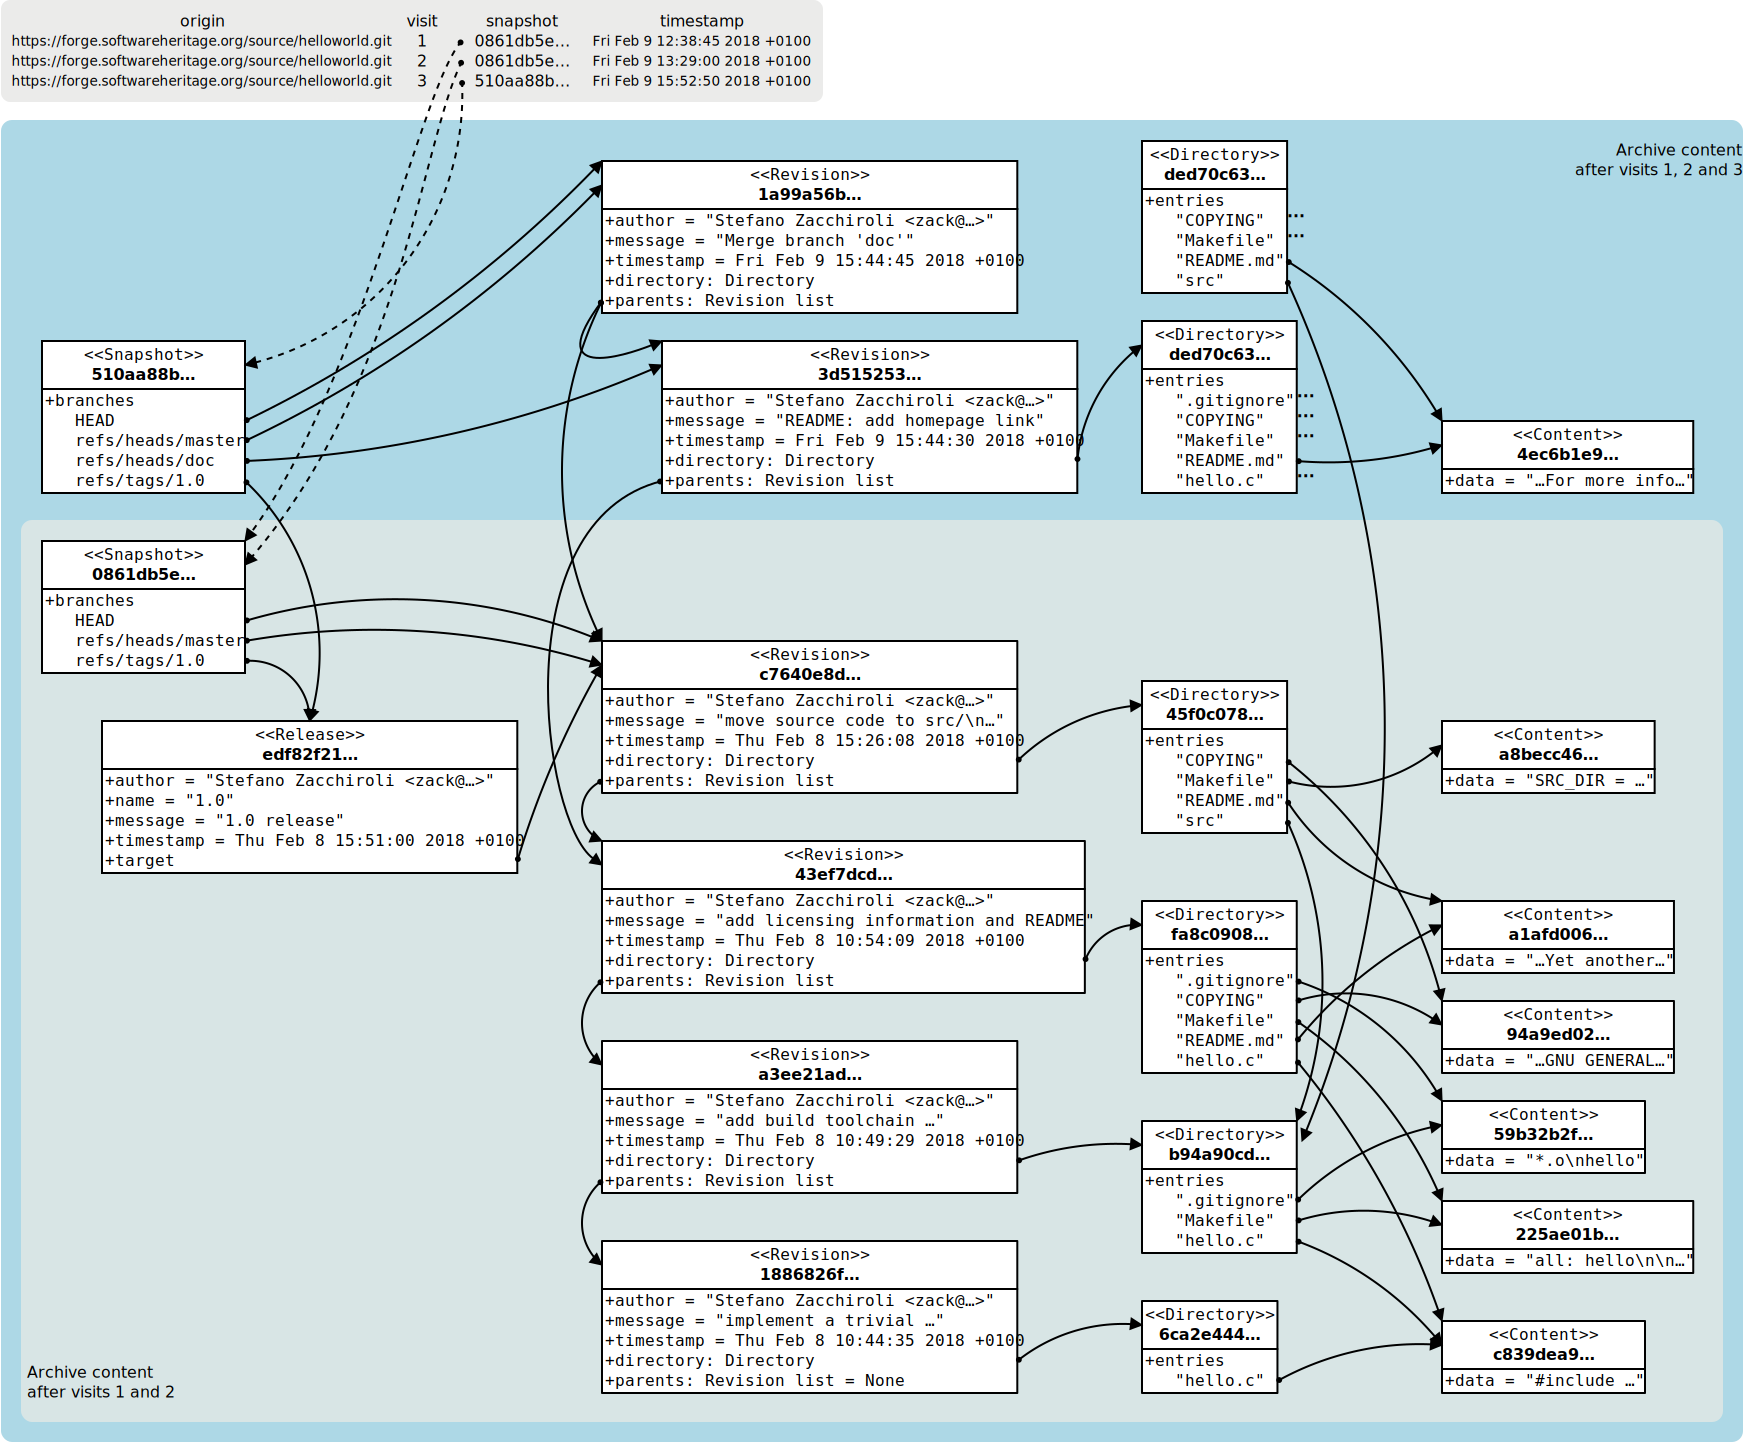
\includegraphics[width=\textwidth]{img/swh-merkle-dag}
    \caption{Detailed view of the Merkle \gls{DAG}, with object contents,
    metadata fields and intrinsic hashes.}%
\end{figure}

The archive is stored as a single large Merkle \gls{DAG}, as depicted
in \cref{fig:swh-model}. In this graph, all software artifacts we have
described correspond to the nodes, which can be of six different types:
blobs, directories, revisions, releases, snapshots and
origins\footnote{Origins are technically not part of the Merkle DAG but rather
only \emph{point} to it, as their intrinsic identifiers are not computed from
their list of descendants, which changes over time.}.
All the nodes are deduplicated and identified by a single intrinsic
identifier, recursively computed from the identifiers of its descendants, which
serves as the primary key in the Merkle \gls{DAG}.

The edges between the nodes of the graph are derived from the relationships
between the artifacts: directory entries point to other directories or file
contents; revisions point to directories and previous revisions; releases point
to revisions; snapshots point to revisions and releases; origins point to the
snapshots that they contained in past visits.
The cardinality diagram shown in \cref{fig:swh-cardinality} formalizes the
different sorts of edges in the graph and their numerical relationships: edges
noted $\prescript{\ast}{}\rightarrow^1$ represent \emph{many-to-one}
relationships (e.g., a revision only points to a single directory, but a
directory can be pointed by multiple revisions) and edges noted
$\prescript{\ast}{}\rightarrow^\ast$ are \emph{many-to-many} relationships
(e.g., a directory can point to multiple blobs, and a single blob can be
pointed by multiple directories).

A few observations can be drawn from this diagram:

\begin{itemize}
    \item Most relationships are many-to-many. Only release $\to$ commit
        and commit $\to$ directory relationships are many-to-one, as
        they can only point respectively to a single commit and a single
        directory.

    \item Commit and directory nodes are parts of recursive relationships.
        Commits point to their parent commits, while directories point to their
        children (sub)directories and files. These two node types are thus what
        gives the DAG an arbitrary depth, as all the other layers have a fixed
        maximum height. Note however that this cycle in the graph cardinality
        diagram does \emph{not} induce cycles in the graph itself, because
        graph nodes are created bottom-up and need to know in advance the
        cryptographic identifiers of target nodes (which thus need to
        exist \emph{before} their parents) in order to be identifiable.

    \item Commits and directories are also mutually recursive, as commits point
        to directories and directories can occasionally point to commits (for
        submodules/externals). This is the only case in which a node can point
        to a node from an upper layer in the cardinality diagram.
\end{itemize}

Note: in the wild one can rarely encounter VCS repositories that contain
unusual relationships between source code artifacts, depicted as dashed arrows
in \cref{fig:swh-cardinality}.
For instance, Git allows you to tag blobs and directories as releases, or to
use blobs as branch destinations.
These are anomalies that in most cases result in non usable VCS data.  We
measured these occurrences in our corpus and verified that they are rare and
unconventional (less than 0.0004\,\% of the total number of edges from releases
and snapshots) and thus, even if they \emph{can} be represented in the \SWH{}
data model, we generally exclude them from our discussion for the sake of
simplicity.

\subsection{Layers}%
\label{sec:layers}

While each relationship can be analyzed independently, it is useful to regroup
the nodes and edges of the Merkle \gls{DAG} by type into logical layers that
are conceptually meaningful.  To that end we define the following subgraphs of
the Software Heritage graph:
\begin{itemize}

\item \emph{Full corpus}: the entire graph of public software development

\item \emph{Filesystem layer}: subset of the full corpus consisting of blob and
  directory nodes only, and edges between them

\item \emph{History layer}: subset of the full corpus consisting of revision and
  release nodes only, and edges between them

\item \emph{Commit layer}: subset of the history layer consisting of revision
  nodes only, and edges between them

\item \emph{Hosting layer}: subset of the full corpus consisting of origins and
  snapshot nodes only, and edges between them

\end{itemize}

\begin{figure}
    \centering
    % 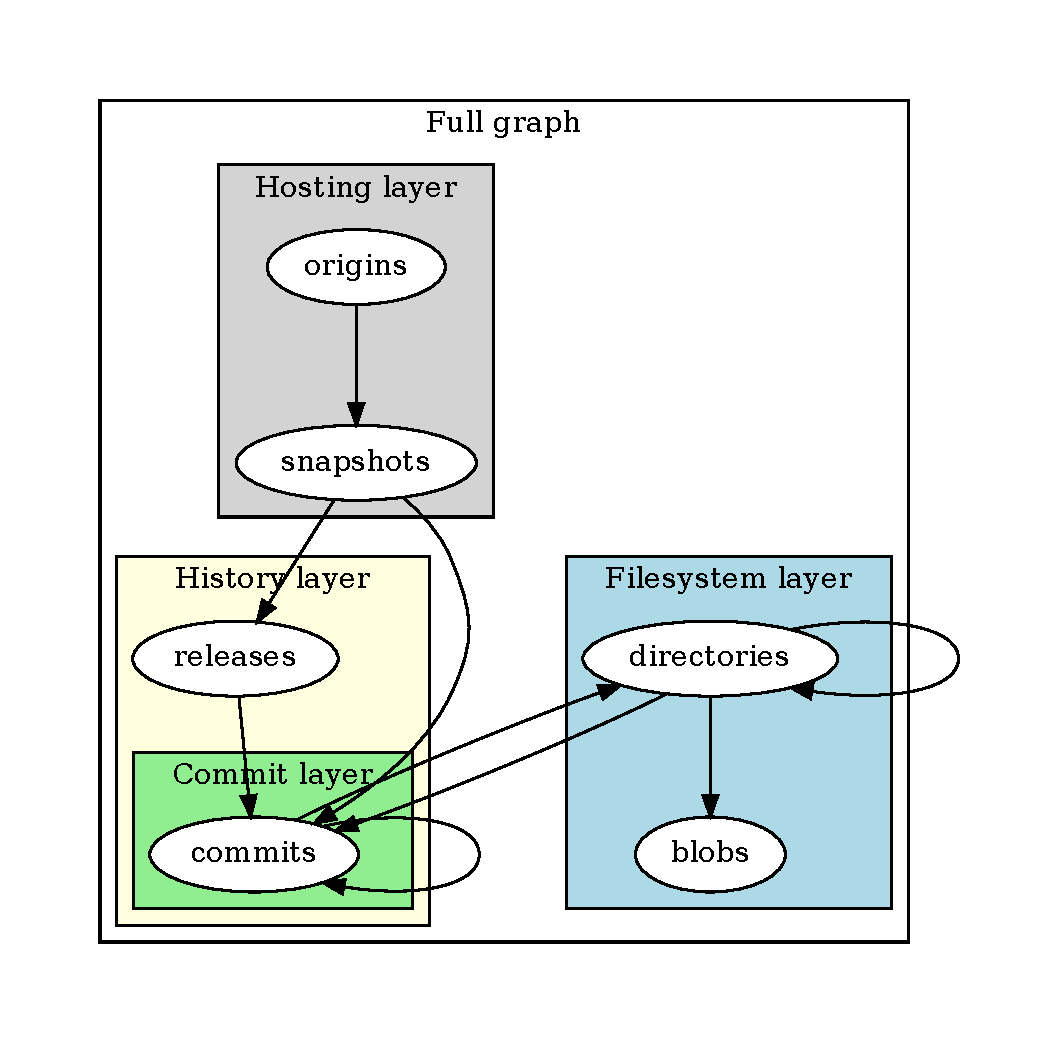
\includegraphics[width=0.6\linewidth,trim=1cm 1cm 1cm 1cm]{img/swh-layers}
    \begin{tikzpicture}[scale=0.8, label distance=1pt]
	\begin{pgfonlayer}{nodelayer}
		\node [draw, shape=ellipse, style=originfill] (origin) at (2, 2) {Origin};
		\node [draw, shape=ellipse, style=snapshotfill] (snapshot) at (2, 0) {Snapshot};
		\node [draw, shape=ellipse, style=releasefill] (release) at (2, -2) {Release};
		\node [draw, shape=ellipse, style=revisionfill] (revision) at (2, -4) {Revision};
		\node [draw, shape=ellipse, style=directoryfill] (directory) at (2, -6) {Directory};
		\node [draw, shape=ellipse, style=contentfill] (content) at (2, -8) {Blob};
		\node [style=none] (1) at (-1.25, -5.25) {};
		\node [style=none] (2) at (4, -5.25) {};
		\node [style=none] (3) at (-1.25, -8.75) {};
		\node [style=none] (4) at (4, -8.75) {};
		\node [style=none] (5) at (-1.25, 2.75) {};
		\node [style=none] (6) at (4, 2.75) {};
		\node [style=none] (7) at (-1.25, -0.75) {};
		\node [style=none] (8) at (4, -0.75) {};
		\node [style=none] (9) at (-1, -3.25) {};
		\node [style=none] (10) at (-1, -4.75) {};
		\node [style=none] (11) at (4, -4.75) {};
		\node [style=none] (12) at (4, -3.25) {};
		\node [style=none] (13) at (-1.25, -1) {};
		\node [style=none] (14) at (7, -1) {};
		\node [style=none] (15) at (-1.25, -5) {};
		\node [style=none] (16) at (7, -5) {};
		\node [style=none] (17) at (-1.5, 3) {};
		\node [style=none] (18) at (-1.5, -9) {};
		\node [style=none] (19) at (10, -9) {};
		\node [style=none] (20) at (10, 3) {};
	\end{pgfonlayer}
	\begin{pgfonlayer}{edgelayer}
		\draw [style=cluster] (5.center) to (6.center);
		\draw [style=cluster] (6.center) to (8.center);
		\draw [style=cluster] (8.center) to (7.center);
		\draw [style=cluster] (5.center) to (7.center);
		\draw [style=cluster] (13.center) to (14.center);
		\draw [style=cluster] (14.center) to (16.center);
		\draw [style=cluster] (16.center) to (15.center);
		\draw [style=cluster] (15.center) to (13.center);
		\draw [style=cluster] (9.center) to (10.center);
		\draw [style=cluster] (10.center) to (11.center);
		\draw [style=cluster] (11.center) to (12.center);
		\draw [style=cluster] (9.center) to (12.center);
		\draw [style=cluster] (1.center) to (3.center);
		\draw [style=cluster] (3.center) to (4.center);
		\draw [style=cluster] (1.center) to (2.center);
		\draw [style=cluster] (2.center) to (4.center);
		\draw [style=cluster] (17.center) to (18.center);
		\draw [style=cluster] (18.center) to (19.center);
		\draw [style=cluster] (19.center) to (20.center);
		\draw [style=cluster] (20.center) to (17.center);
		\draw [style=arrow] (origin) to (snapshot);
		\draw [style=arrow] (snapshot) to (release);
		\draw [style=arrow] (release) to (revision);
		\draw [style=arrow] (revision) to (directory);
		\draw [style=arrow] (directory) to (content);
		\draw [style=dashed arrow, draw=lightgray, bend right=60, looseness=0.75] (snapshot) to (content);
		\draw [style=dashed arrow, draw=lightgray, bend right=60, looseness=0.75] (snapshot) to (directory);
		\draw [style=dashed arrow, draw=lightgray, bend right=45] (release) to (directory);
		\draw [style=dashed arrow, draw=lightgray, bend right=45] (release) to (content);
		\draw [style=arrow, loop left, loop] (revision) to ();
		\draw [style=arrow, bend right] (directory) to (revision);
		\draw [style=arrow, loop left, loop] (directory) to ();
		\draw [style=arrow, bend right=60] (snapshot) to (revision);

        \draw [decorate, decoration={brace,raise=5pt,amplitude=10pt}] (6) to node [align=left, right=20pt, style=none] {Hosting\\ layer} (8);
        \draw [decorate, decoration={brace,raise=5pt,amplitude=5pt}] (12) to node [align=left, right=20pt, style=none] {Commit\\ layer} (11);
        \draw [decorate, decoration={brace,raise=5pt,amplitude=10pt}] (2) to node [align=left, right=20pt, style=none] {Filesystem\\ layer} (4);
        \draw [decorate, decoration={brace,raise=5pt,amplitude=10pt}] (14) to node [align=left, right=20pt, style=none] {History\\ layer} (16);
        \draw [decorate, decoration={brace,raise=5pt,amplitude=10pt}] (20) to node [align=left, right=20pt, style=none] {Full graph} (19);
	\end{pgfonlayer}
\end{tikzpicture}

    \caption{Logical layers used to refer to specific subsets of the graph.}%
    \label{fig:layers}
\end{figure}
\Cref{fig:layers} shows the various layers, which types of nodes belong to
each of them, as well as how edges connect them. In later chapters, we will
study properties of both the full graph of public software development and of
the specific subgraphs named above.


\subsection{Persistent identifiers}%
\label{sec:swhid}

The intrinsic hashes used to identify the nodes can be used to provide a
standardized and portable way of referring to the artifacts in the
archive~\cite{swhipres2018}. This is achieved by \glspl{SWHID},
% (IPA: /swiːd/)
short strings that identify a single object and which are guaranteed to remain
stable over time.  These identifiers were introduced by
\textcite{cise-2020-doi} and are documented in the Software Heritage
development
documentation\footnote{\url{https://docs.softwareheritage.org/devel/swh-model/persistent-identifiers.html}}.
\glspl{SWHID} are represented in the following basic syntax:

\texttt{swh:<scheme version>:<object type>:<object id>}

The current version of the identifier scheme, stored in the second field, is
\texttt{1}. The third field contains a three-letter code for the object type
(\texttt{snp} for snapshots, \texttt{rel} for releases, \texttt{rev} for
revisions, \texttt{dir} for directories and \texttt{cnt} for file contents).
The last field contains an intrinsic hash computed with the SHA-1 algorithm on
the content and metadata of the object and encoded in hexadecimal.

Here are a few examples of \glspl{SWHID} and the objects they point to:

\begin{itemize}
    \setlength\itemsep{0em}
    \item \texttt{swh:1:cnt:94a9ed024d3859793618152ea559a168bbcbb5e2} points to
        the content of a file containing the full text of the GPL-3 license.
    \item \texttt{swh:1:rev:309cf2674ee7a0749978cf8265ab91a60aea0f7d} points to
        a revision in the development history of the Darktable photography
        application.
    \item \texttt{swh:1:snp:c7c108084bc0bf3d81436bf980b46e98bd338453} points to
        a snapshot of the entire Git repository of Darktable as of May 4, 2017.
\end{itemize}

\glspl{SWHID} have interesting uses for research replicability: studies
citing software by URL can be subject to \emph{link rot}, which could make it
harder to run the software again as a way to independently verify the study
results. Because \glspl{SWHID} are persistent, using these identifiers to cite
scientific software is a way to ensure that the citation remains unambiguous
and resilient to URL changes. \glspl{SWHID} can be computed independently and
do not require a centralized authority for allocation, as they are solely
computed from the intrinsic properties of the object they refer to.

\section{Implementation}%
\label{sec:swh-infrastructure}

Although a full description of the physical infrastructure powering the
Software Heritage archive is out of scope for this thesis, a cursory
understanding of some of its core systems is needed for later chapters, as we
present frameworks and tools built upon these foundations.

At a physical level, the archive is stored using a few different technologies,
due to the differences in technical requirements for storing the different
layers of the graph~\cite{swhipres2017}.
Most notably, the source file contents require orders of magnitude more space
($\approx 850$ TiB as of May 2021) than the rest of the archive and are thus
stored on dedicated key-value object storage systems, keyed by their intrinsic
hash.  In the infrastructure hosted in-house by the Software Heritage
initiative, the object hashes allow for efficient horizontal sharding, by
assigning hash prefixes to specific servers. This technique is used to
trivially implement a reasonably performant and redundant storage.
Key-value object storage systems are an almost universal primitive in cloud
offerings, which allows Software Heritage to store an entire copy of the
blob layer in two different clouds: the Microsoft Azure Blob Storage and
Amazon AWS S3.

On the other hand, the upper layers of the archive require significantly less
storage space ($\approx 10$ TiB) but have different functional requirements, as
they have more associated metadata (author names, revision messages, children
nodes, …) that need to be made searchable and joinable. This part of the graph
is stored in a \gls{RDBMS}, where nodes and edges have a few associated
relational tables that describe it. These systems can be leveraged to build
indexes, e.g., on the hashes stored in the different fields, which can then be
used to randomly access specific nodes and edges, and to efficiently
\emph{join} tables together to combine data from multiple node types by
following their links.

This approach can have scalability issues, as inserting data in traditional
\glspl{RDBMS} gets exponentially slower as the tables grow.  Other storage
systems for the graph are under study to circumvent this problem, notably the
use of key-value document storage systems like Cassandra or ScyllaDB\@.

One last relevant component is the \emph{journal}, which serves as a
synchronization pipeline across the infrastructure. In order to keep the
variety of storage backends (object storage, database, document stores…)
consistent together, the journal acts as a persistent log of the archive, where
all the ingested objects are pushed in order. All the backends and their
replicas can then subscribe to the journal and read its messages to keep
themselves up-to-date with the current state of the archive.
